\section{CI/CD và End-to-End Testing}

\subsection{CI/CD Pipeline}

Dự án sử dụng GitHub Actions để tự động hóa quá trình testing và deployment.

\subsubsection{Workflow Configuration}

\begin{lstlisting}[language=yaml, caption=GitHub Actions CI/CD Config]
name: Complete CI Pipeline

on:
  push:
    branches: [ "**" ]
  pull_request:
    branches: [ "**" ]

jobs:
  complete-ci:
    runs-on: ubuntu-latest
    services:
      mysql:
        image: mysql:8.0
        env:
          MYSQL_DATABASE: flogin_db
          MYSQL_USER: flogin
          MYSQL_PASSWORD: flogin123
          MYSQL_ROOT_PASSWORD: root123
        ports:
          - 3306:3306
    strategy:
      matrix:
        java-version: [ '21' ]
        node-version: [ '20' ]
    steps:
      - name: Checkout source
        uses: actions/checkout@v4
      - name: Set up JDK ${{ matrix.java-version }}
        uses: actions/setup-java@v4
        with:
          distribution: 'temurin'
          java-version: ${{ matrix.java-version }}
          cache: maven
      - name: Backend - run tests
        working-directory: backend
        run: mvn -B clean test
      - name: Set up Node.js ${{ matrix.node-version }}
        uses: actions/setup-node@v4
        with:
          node-version: ${{ matrix.node-version }}
          cache: 'npm'
      - name: Frontend - install dependencies
        working-directory: frontend
        run: npm ci
      - name: Frontend - unit tests with coverage
        working-directory: frontend
        run: npm test -- --watch=false --coverage
      - name: Frontend - build production
        working-directory: frontend
        run: CI=false npm run build
\end{lstlisting}

\begin{figure}[H]
\centering
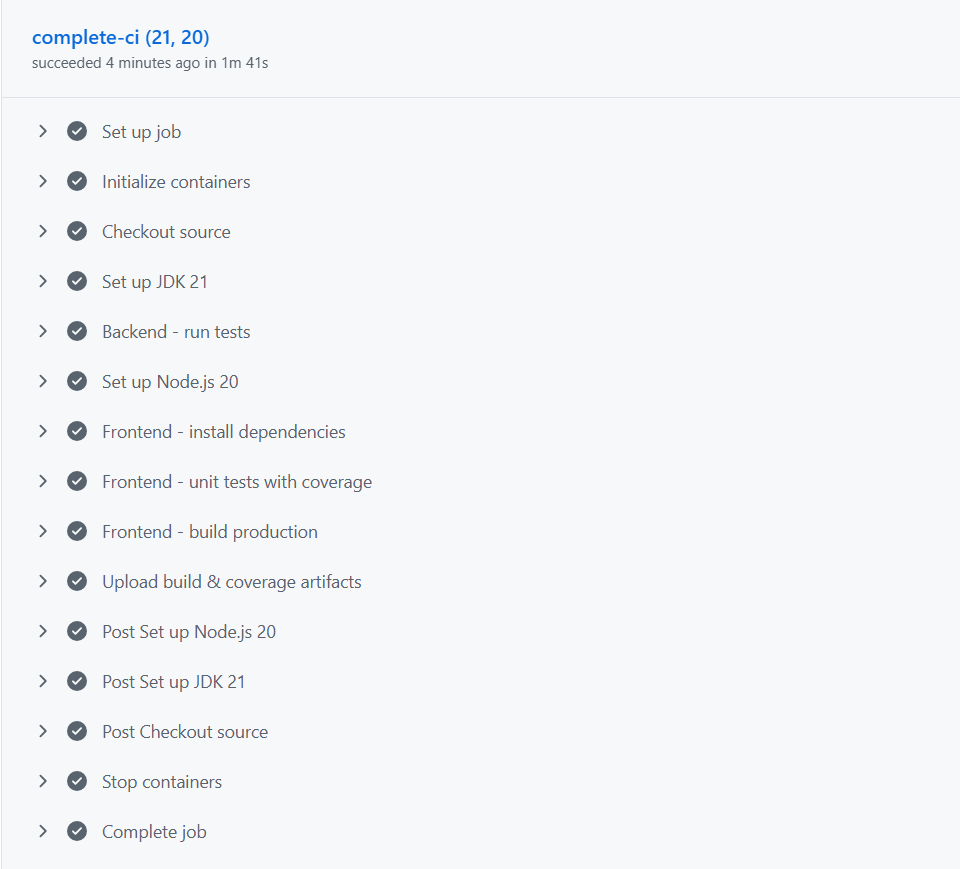
\includegraphics[width=1.0\textwidth]{images/CICD/CICDfull.png}
\caption{Complete CI Pipeline - GitHub Actions Workflow Results}
\end{figure}

\subsection{End-to-End Testing với Cypress}

\subsubsection{Cypress Configuration}

\begin{lstlisting}[language=JavaScript, caption=Cypress Configuration]
const { defineConfig } = require("cypress");

module.exports = defineConfig({
  e2e: {
    baseUrl: 'http://localhost:3000',
    
    setupNodeEvents(on, config) {
      // Noi cau hinh cac plugin hoac su kien lang nghe
    },
  },
});
\end{lstlisting}

\subsubsection{E2E Test Cases}

\begin{lstlisting}[language=JavaScript, caption=Login E2E Test]
describe('Login E2E Tests', () => {
  beforeEach(() => {
    cy.visit('http://localhost:3000/login');
  });

  it('d) Nen hien thi day du cac UI elements', () => {
    cy.get('[data-testid="username-input"]').should('be.visible');
    cy.get('[data-testid="password-input"]').should('be.visible');
    cy.get('[data-testid="login-button"]').should('be.visible');
    cy.contains('h2', 'Dang Nhap').should('be.visible');
  });

  it('b) Nen hien thi validation error khi submit form rong', () => {
    cy.get('[data-testid="login-button"]').click();
    cy.contains('Username khong duoc de trong').should('be.visible');
    cy.contains('Password khong duoc de trong').should('be.visible');
  });

  it('c) Nen hien thi loi khi login fail', () => {
    cy.intercept('POST', 'http://localhost:8080/api/auth/login', {
      statusCode: 401,
      body: { success: false, message: 'Ten dang nhap hoac mat khau khong dung!' }
    }).as('loginFail');
    cy.get('[data-testid="username-input"]').type('wronguser');
    cy.get('[data-testid="password-input"]').type('Wrong123');
    cy.get('[data-testid="login-button"]').click();
    cy.wait('@loginFail');
    cy.contains('Ten dang nhap hoac mat khau khong dung!').should('be.visible');
  });

  it('a) Nen login thanh cong voi credentials hop le', () => {
    cy.intercept('POST', 'http://localhost:8080/api/auth/login', {
      statusCode: 200,
      body: {
        success: true,
        data: { token: 'fake-jwt-token', user: { id: 1, username: 'testuser' } }
      }
    }).as('loginSuccess');
    cy.get('[data-testid="username-input"]').type('testuser');
    cy.get('[data-testid="password-input"]').type('Test123');
    cy.get('[data-testid="login-button"]').click();
    cy.wait('@loginSuccess');
    cy.url().should('include', '/products');
  });
});
\end{lstlisting}

\subsubsection{Product Management E2E Test}

\begin{lstlisting}[language=JavaScript, caption=Product E2E Test - CRUD Operations]
import ProductPage from '../support/pages/ProductPage.js';

describe('Product Management E2E Tests', () => {
  const productPage = new ProductPage();
  const timestamp = Date.now();
  const testProduct = {
    name: `Iphone Test ${timestamp}`,
    price: '20000000',
    quantity: '100',
    category: 'Test Device'
  };

  beforeEach(() => {
    cy.login('testuser', 'admin123');
    productPage.visit();
  });

  it('A. Should create a new product successfully', () => {
    productPage.clickAddNew();
    cy.get('.modal-content').should('be.visible');
    productPage.fillProductForm(testProduct);
    productPage.submitForm();
    cy.get('.modal-content').should('not.exist');
    cy.contains('.product-card', testProduct.name).should('be.visible');
  });

  it('B. Should display product list', () => {
    cy.get('.products-grid').should('exist');
    cy.get('.product-card').should('have.length.greaterThan', 0);
  });

  it('E. Should search for the product correctly', () => {
    productPage.searchProduct(testProduct.name);
    cy.contains('.product-card', testProduct.name).should('be.visible');
  });

  it('C. Should update the product price', () => {
    productPage.visit();
    const newPrice = '25000000';
    productPage.clickEditProduct(testProduct.name);
    cy.get('#product-price').should('be.visible').clear().type(newPrice);
    productPage.submitForm();
    cy.contains('.product-card', testProduct.name).should('contain', '25');
  });

  it('D. Should delete the product', () => {
    productPage.visit();
    productPage.acceptDeleteConfirmation();
    productPage.clickDeleteProduct(testProduct.name);
    cy.contains('.product-card', testProduct.name).should('not.exist');
  });
});
\end{lstlisting}

\subsubsection{Login Tests CI Workflow}

\begin{lstlisting}[language=yaml, caption=Login-specific CI Pipeline]
name: Login Tests CI

on:
  push:
    branches: ["**"]
  pull_request:
    branches: ["**"]

jobs:
  test-login:
    runs-on: ubuntu-latest

    defaults:
      run:
        working-directory: ./frontend

    steps:
      - name: Checkout source
        uses: actions/checkout@v4

      - name: Setup Node.js
        uses: actions/setup-node@v4
        with:
          node-version: '20'
          cache: npm
          cache-dependency-path: frontend/package-lock.json

      - name: Install dependencies
        run: npm ci

      # Unit test cho phan Login
      - name: Run Login unit tests
        run: npm test -- --testPathPattern=Login

      # E2E login voi Cypress
      - name: Run Login E2E tests (Cypress)
        run: npm run test:e2e -- --spec "cypress/e2e/login.e2e.spec.cy.js"
\end{lstlisting}

\begin{figure}[H]
\centering
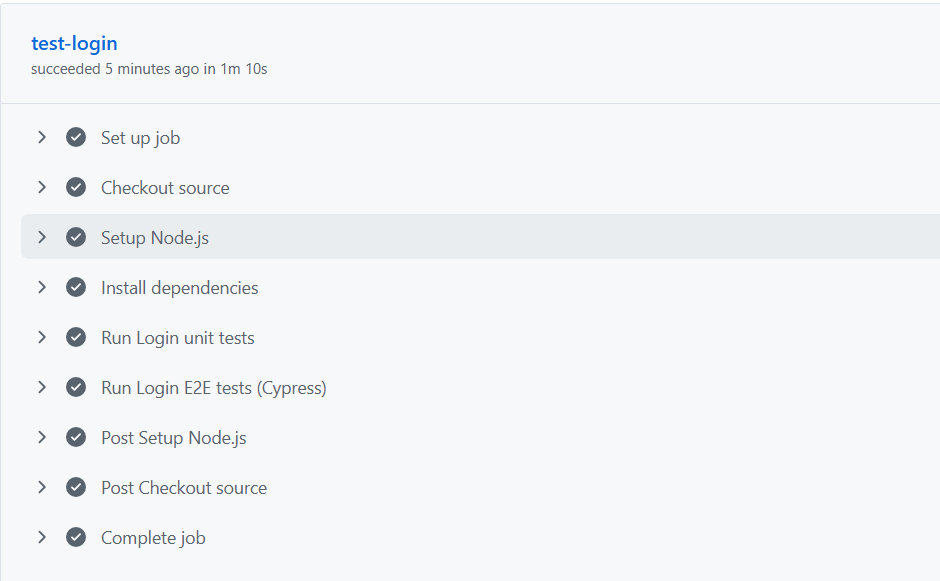
\includegraphics[width=1.0\textwidth]{images/CICD/CICDlogin.png}
\caption{Login Tests CI Pipeline - Specialized Workflow Results}
\end{figure}

\subsection{CI/CD Pipeline Details}

\subsubsection{Complete CI Workflow}

Pipeline bao gom cac stages:

\begin{enumerate}
    \item \textbf{Source Checkout}: Lay code tu repository
    \item \textbf{Environment Setup}:
    \begin{itemize}
        \item MySQL service container (port 3306)
        \item Java 21 (Temurin distribution)
        \item Node.js 20
        \item Maven va npm caching
    \end{itemize}
    \item \textbf{Backend Testing}:
    \begin{itemize}
        \item Run all unit tests: \texttt{mvn -B clean test}
        \item Connect to MySQL service
        \item Environment variables for database connection
    \end{itemize}
    \item \textbf{Frontend Testing}:
    \begin{itemize}
        \item Install dependencies: \texttt{npm ci}
        \item Run unit tests with coverage: \texttt{npm test --watch=false --coverage}
        \item Build production: \texttt{CI=false npm run build}
    \end{itemize}
    \item \textbf{Artifacts Upload}:
    \begin{itemize}
        \item Backend: \texttt{backend/target}
        \item Frontend: \texttt{frontend/build}, \texttt{frontend/coverage}
    \end{itemize}
\end{enumerate}

\subsubsection{CI/CD Triggers}

\begin{itemize}
    \item \textbf{Push}: Bat ky branch nao (\texttt{branches: ["**"]})
    \item \textbf{Pull Request}: Bat ky branch nao
    \item \textbf{Auto-run}: Moi khi co thay doi code
\end{itemize}

\subsubsection{Matrix Strategy}

\begin{itemize}
    \item Java versions: [21]
    \item Node versions: [20]
    \item Co the mo rong: Them nhieu versions de test compatibility
\end{itemize}

\subsubsection{Specialized Workflows}

Du an co 2 workflows chinh:

\begin{enumerate}
    \item \textbf{Complete CI Pipeline} (\texttt{ci.yml}):
    \begin{itemize}
        \item Chay tat ca backend tests (Unit + Integration)
        \item Chay tat ca frontend tests (Unit + E2E)
        \item Build production artifacts
        \item Upload coverage reports
        \item Working directory: root (kiem soat ca backend va frontend)
    \end{itemize}
    
    \item \textbf{Login Tests CI} (\texttt{login-tests.yml}):
    \begin{itemize}
        \item Focus chi vao Login functionality
        \item Chay Login unit tests: \texttt{npm test -- --testPathPattern=Login}
        \item Chay Login E2E tests: \texttt{cypress/e2e/login.e2e.spec.cy.js}
        \item Working directory: \texttt{./frontend}
        \item Nhanh hon, chi test Login component
    \end{itemize}
\end{enumerate}

\textbf{Loi ich cua 2 workflows:}
\begin{itemize}
    \item \textbf{Complete CI}: Bao dam toan bo he thong hoat dong
    \item \textbf{Login Tests}: Kiem tra nhanh khi sua doi Login (faster feedback)
    \item \textbf{Parallel execution}: Co the chay dong thoi tren cac branches khac nhau
    \item \textbf{Selective testing}: Developer chi chay workflow can thiet
\end{itemize}

\subsection{Ket qua CI/CD}

\begin{itemize}
    \item \textbf{Complete CI}: Tat ca tests chay tu dong khi push code (~3-5 phut)
    \item \textbf{Login Tests CI}: Login-specific tests (~1-2 phut)
    \item Test coverage duoc report tu dong
    \item Phat hien loi som trong qua trinh development
    \item Artifacts (build files, coverage) duoc luu lai de review
\end{itemize}

\subsection{CI/CD Best Practices}

\begin{itemize}
    \item \textbf{Caching}: Maven va npm dependencies duoc cache
    \item \textbf{Service Containers}: MySQL chay trong Docker container
    \item \textbf{Matrix Testing}: Co the test tren nhieu versions
    \item \textbf{Parallel Jobs}: Frontend va Backend tests co the chay parallel
    \item \textbf{Fail Fast}: Pipeline dung ngay khi co loi
    \item \textbf{Artifacts}: Luu build results va coverage reports
\end{itemize}
